Le rapport à mi-parcours contient
\begin{itemize}
\item un calendrier prévisionnel précis et réaliste pour la troisième année et jusqu’à la soutenance de la thèse,
\item un CV (liste de publications, responsabilités, enseignement,…),
\item un bilan des formations suivies et prévues (extrait du compte personnel ADUM),
\item rapport à mi-parcours (y compris l'état de l'art, reprise des 2+1 articles accompagnés d'une présentation générale).
\end{itemize}

\section*{Calendrier prévisionnel pour la troisième année}
Date de la 1ere inscription en thèse: 28 octobre 2016\\
Date de soutenance prévue: septembre 2019\\

\begin{table}[ht]
\begin{center}
\begin{tabular}{r|c|c}
Dates & Task & Details\\ \hline
Aug`18 & Finish implementation work & Complete end-to-end system\\
Sep`18 & First evaluation/experiments & User studies with end-to-end system\\
Oct`18 &Improve framework based on first experiments & Adjust program flow \\
Nov`18 & Second evaluation/experiments & User studies with improved system\\
Dec`18 & \textit{Buffer month} & Finish all experiments and evaluations\\
 & & Write paper for IJCAI`19\\ \hline
Jan`19 & Start full-time thesis write-up & Thesis state is 30\% of content \\
Feb`19 & 1st draft (to be reviewed by supervisors) & $\geq 60\%$ + add more content \\
Mar`19 & 2nd draft & $\geq80\%$ + structural changes \\
Apr`19 & 3rd draft & $\geq 90\%$ + structural changes only \\
May`19 & Final draft & Make final edits/modifications\\
 & Hand in thesis & Final submission of thesis to the jury\\
Sep`19 & \textbf{Thesis defence} & \\
\end{tabular}
\end{center}
\end{table}

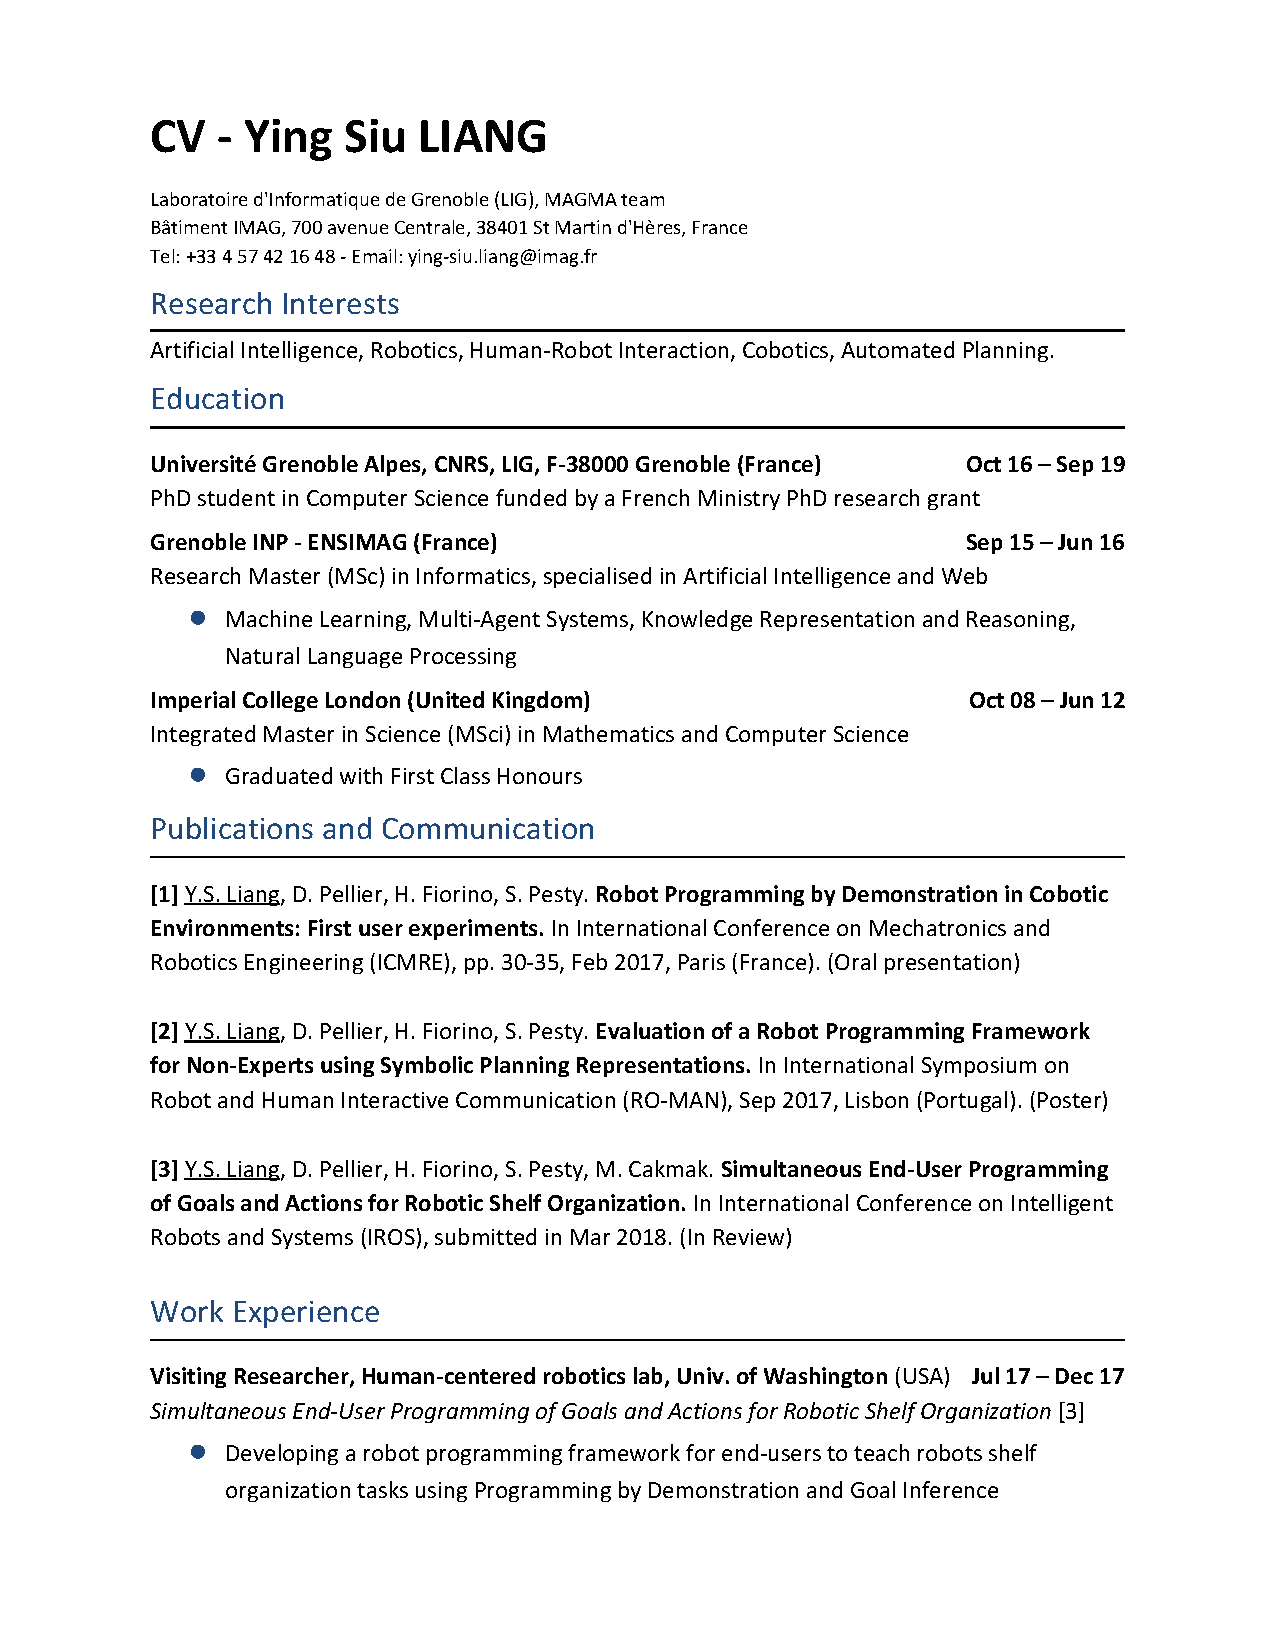
\includepdf[pages=1-2]{0-frontmatter/CV.pdf}
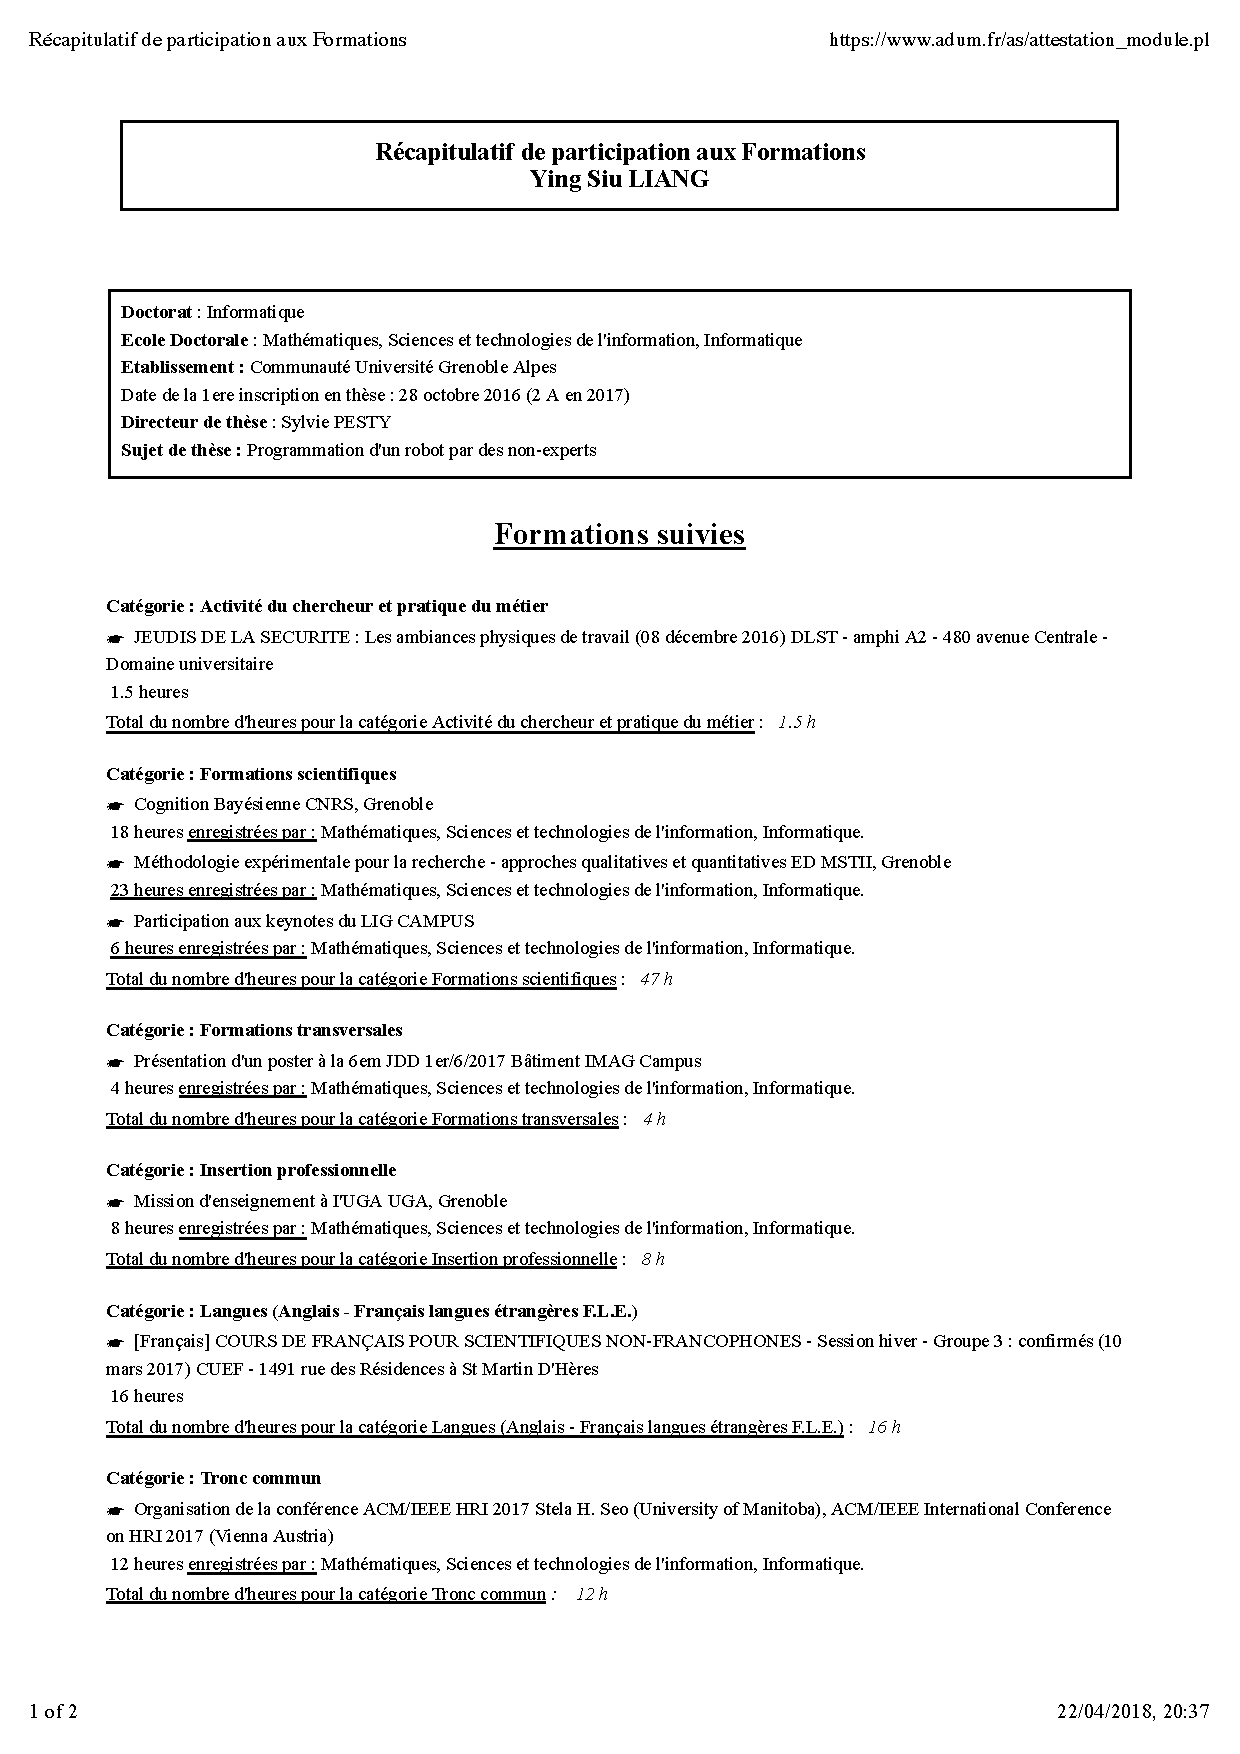
\includepdf[pages=1-2]{0-frontmatter/validated-credits.pdf}